\documentclass[main.tex]{subfiles}

\begin{document}

	\begingroup

	\renewcommand{\cleardoublepage}{}

	\renewcommand{\clearpage}{}

	\chapter{Cleanup Task Overview}

		\chapterauthor{Torge Olliges}
		
		\section{Goal}
		For the cleanup task the HSR had to navigate a room in which objets are distributed. The robot has no prior knowledge of the position of the objects but it does know the position of the goal which was ....... It had to be able to detect the objects in the room pick them up and transport them to the designated goal position. The HSR had to achieve the tasks given autonomusly and manipulate objects like the objects explained in the goal section of the gorcery task chapter. It had 5 minutes to achieve this task.
		
		\section{Architecture}
		
		\section{Description}
	  	
	  	\section{Tasks}
	  	\begin{figure}	
	  		\centering
	  		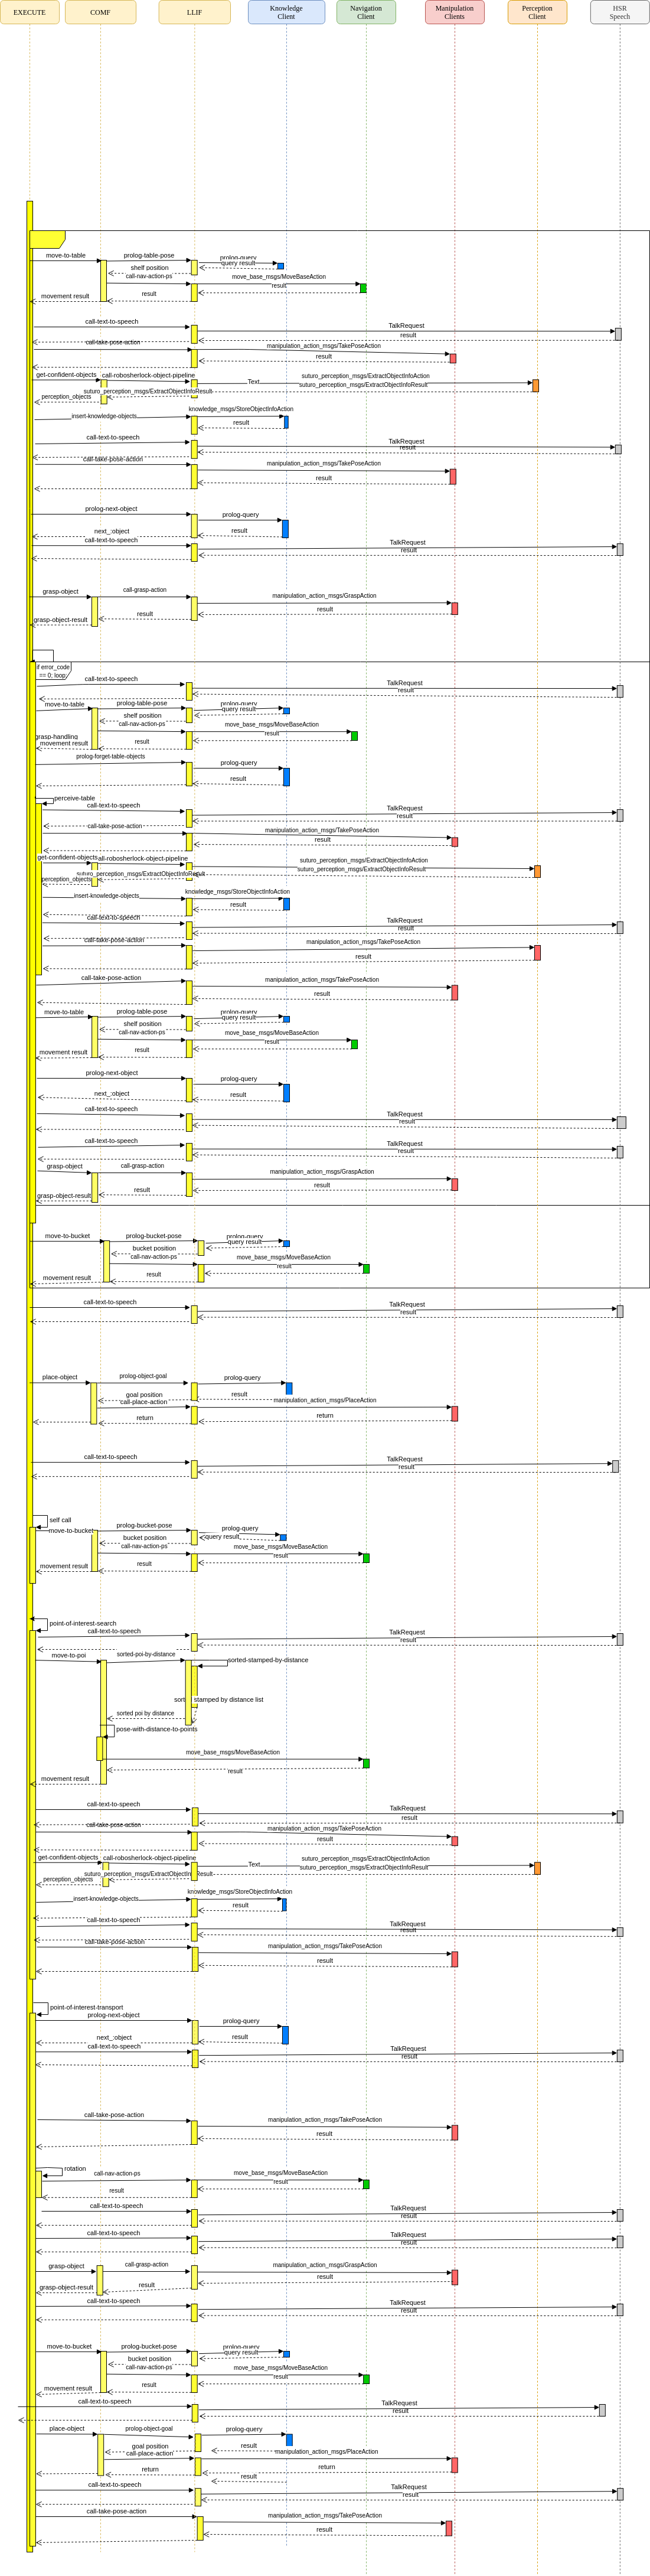
\includegraphics[width=0.85\textwidth]{pictures/diagramms/cleanup-sequence.png}
	  		\caption{Sequence diagram of the complete run of the clean up task \textit{(explanations below)}}
	  		\label{cleanup-sequence}
	  	\end{figure}
		hier bitte aus dem sequenz diagramm einen einzelnen task als subsection z.b. schritt: tür öffnen, dafür mussten perception dies tun manipulation das tun etc.
		
		\subsection{startup sequence}
	First the interface to knowledge is called to set the target to basket. In addition, the floor and the table are set as sources, since objects are picked up from both. Since knowledge is responsible for the internal representation of the surfaces and the management of the associated objects, we have to tell them from where we will pick up objects and where they will be taken. 

	\subsection{perceive table sequence}
	To scan the table, the robot is moved to the table. This is done with a position of the table given by Knowlege. After that, manipulation is given the command to go into the perceive pose, so that the table is well visible in the camera image. Then perception is called, so that they can process the current camera image. The region of the table is also passed to Perception so that Perception can apply a region filter.

	\subsection{grasp sequence}
	\subsection{travel sequence}
	\subsection{place sequence}
	\subsection{point of interest search sequence}
	\subsection{point of interest grasp sequence}
	\subsection{point of interest place sequence}


		
		\section{Conclusion}
		
		
	\endgroup

\end{document}
